\iffalse
\chapter{2024}
\author{EE24BTECH11015 - Dhawal}
\section{xe}
\fi


\item The axial velocity profile of a laminar, incompressible and fully-developed flow in a circular pipe of radius ($ R $) is given as 
\begin{align*}
    u_z = -\frac{1}{4\mu} \frac{\partial p}{\partial z} R^2 \brak{ 1 - \frac{r^2}{R^2} },
\end{align*}  
where $r, z, \mu, $ and $ p $ are radial direction, axial direction, fluid viscosity, and pressure, respectively. If the average velocity of the flow is given by 
\begin{align*}
    u_{z,\text{avg}} = \frac{1}{K} \brak{ -\frac{R^2}{\mu} \frac{\partial p}{\partial z} }, 
\end{align*} 
then the value of $ K $ (answer in integer) is 
 \rule{1cm}{0.4 pt}


\item The velocity potential function in a two-dimensional flow field is given by\\
$ \Phi\brak{x, y} = -\brak{axy + bx^2 - by^2} \, \text{m}^2/\text{s} \quad \text{where} \, a = 2 \, \text{per second} \, \text{and} \, b = 0.5 \, \text{per second}. $
The magnitude of the velocity (in m/s, answer in integer) at $ x = 2 \, \text{m}, y = 1 \, \text{m} $ is \rule{1cm}{0.4 pt}.



\item Consider the incompressible, steady and irrotational flow through a concentric reducer in a horizontal pipeline. The pipe diameter reduces from $ d_1 = 12 \, \text{cm} $ to $ d_2 = 4 \, \text{cm} $ as shown in figure. The pressure at position $1$ and position $2$ of the reducer is $ p_1 = 55 \, \text{kPa} $ and $ p_2 = 27 \, \text{kPa}$, respectively. The specific weight of fluid is $ 7 \, \text{kN/m}^3 $. Acceleration due to gravity is $ 10 \, \text{m/s}^2 $.

\begin{center}
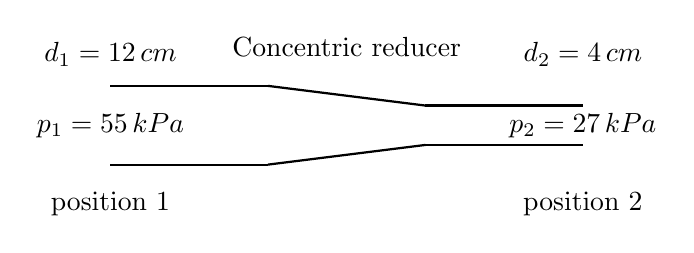
\begin{tikzpicture}
    % Draw the concentric reducer
    \draw [thick] (0,0) -- (2,0);
    \draw [thick] (0,1) -- (2,1);
    \draw [thick] (2,0) -- (4,0.25);
    \draw [thick] (2,1) -- (4,0.75);
    \draw [thick] (4,0.25) -- (6,0.25);
    \draw [thick] (4,0.75) -- (6,0.75);

    % Label positions
    \node at (0,-0.5) {position 1};
    \node at (6,-0.5) {position 2};
    \node at (3, 1.5) {Concentric reducer};

    % Draw dimensions
    
    \node at (0, 1.4) {$d_1 = 12 \, \text{cm}$};
    
    \node at (6, 1.4) {$d_2 = 4 \, \text{cm}$};

    % Draw pressures
    \node at (0, 0.5) {$p_1 = 55 \, \text{kPa}$};
    \node at (6, 0.5) {$p_2 = 27 \, \text{kPa}$};
\end{tikzpicture}
\end{center}

Neglecting frictional effects, the mass flow rate (in kg/s, rounded off to two decimal places) of the fluid through the reducer is \rule{1cm}{0.4 pt}.


\item Consider the incompressible fluid flow over a flat plate with a free stream velocity, $ U_\infty = 1 \, \text{m/s} $. The fluid kinematic viscosity is $ 10^{-6} \, \text{m}^2/\text{s} $ and density is $ 1 \, \text{kg/m}^3 $. The velocity profile within the boundary layer at any location $ x $ is given by\\
$ u(y) = U_\infty \brak{ \frac{3}{2} \frac{y}{\delta} - \frac{1}{2} \brak{ \frac{y}{\delta} }^3 }, $
where boundary layer thickness,
$ \delta = \frac{4.64x}{\sqrt{R_\text{ex}}}, \quad \text{and} \quad R_\text{ex} = \frac{U_\infty x}{\nu}. $
The local wall shear stress at $ x = 1 \, \text{m} $ from the leading edge is \rule{1cm}{0.4 pt} $\times 10^{-3} \, \text{N/m}^2 $ (rounded off to two)

\item The correct combination of phases in the one-component H$_2$O phase diagram, as given below, is

\begin{center}
\begin{circuitikz}[scale=0.51]
\tikzstyle{every node}=[font=\normalsize]

\draw [short] (3.25,6.75) .. controls (5,7.25) and (5,7.25) .. (5.75,8.75);
\draw [short] (5.75,8.75) .. controls (7.25,9.25) and (7.5,9) .. (8,10.25);
\draw [short] (5.75,8.75) .. controls (4.5,9.25) and (4.25,9.5) .. (4,10.75);
\draw [->, >=Stealth] (2.75,6.5) .. controls (6.25,6.5) and (6,6.5) .. (9.25,6.5) ;
\draw [->, >=Stealth] (2.75,6.5) .. controls (2.75,8.75) and (2.75,9) .. (2.75,11.75) ;
\node [font=\large] at (8.5,6) {T};
\node [font=\large] at (2,11) {P};
\node [font=\normalsize] at (7,8) {$\gamma$};
\node [font=\normalsize] at (4.25,8.5) {$\alpha$};
\node [font=\normalsize] at (6,10) {$\beta$};
\end{circuitikz}
\end{center}

\begin{multicols}{2}
\begin{enumerate}
\item $ \alpha $ -- water; $ \beta $ -- vapour; $ \gamma $ -- ice 
\item $ \alpha $ -- ice; $ \beta $ -- water; $ \gamma $ -- vapour
\item $\alpha $ -- vapour; $ \beta $ -- ice; $ \gamma $ -- water
\item $\alpha $ -- water; $ \beta $ -- ice; $ \gamma $ -- vapour
\end{enumerate}
\end{multicols}

\item Mechanical behaviour of a crystalline ceramic material is best described as

\begin{multicols}{4}
\begin{enumerate}
\item ductile
\item brittle
\item viscoelastic
\item viscoplastic
\end{enumerate}
\end{multicols}

\item Differential scanning calorimetry involves measurement of 
\begin{multicols}{4}
\begin{enumerate}
\item weight change
\item entropy 
\item heat 
\item vapour pressure
\end{enumerate}
\end{multicols}

\item In ball milling of ceramic powder, selection of grinding media depends on the
\rule{1cm}{0.4 pt} difference between grinding media and powder particles. 
\begin{multicols}{2}
\begin{enumerate}
\item thermal conductivity 
\item dielectric constant
\item hardness
\item density
\end{enumerate}
\end{multicols}

\item Which one of the following unit cell parameters represents a tetragonal crystal
system? 
\begin{multicols}{2}
\begin{enumerate}
\item $a = b = c ; \alpha=  \beta=  \gamma\neq  90\degree $
\item $a \neq b \neq c ; \alpha=  \beta=  \gamma=  90\degree $
\item $a = b \neq c ; \alpha=  \beta=90\degree,  \gamma=  120\degree $
\item $a = b \neq c ; \alpha=  \beta=  \gamma=  90\degree $
\end{enumerate}
\end{multicols}

\item Which of the following types of materials exhibit(s) positive magnetic
susceptibility? 
\begin{multicols}{4}
\begin{enumerate}
\item Paramagnetic 
\item Diamagnetic 
\item Ferrimagnetic
\item Ferromagnetic
\end{enumerate}
\end{multicols}

\item Which of the following is/are responsible for pitting corrosion in a metal ?
\begin{multicols}{2}
\begin{enumerate}
\item Rough surface
\item Grain boundaries 
\item Polished surface 
\item Polymer coated metal surface
\end{enumerate}
\end{multicols}

\item In thermogravimetric analysis (TGA), weight change of a material sample during
decomposition with temperature is shown in the figure below. 
\begin{center}
    \begin{circuitikz}[scale=0.74]
\tikzstyle{every node}=[font=\normalsize]
\draw [short] (2,9.5) .. controls (3.25,9.5) and (3,9.5) .. (4,9.5);
\draw [short] (5,8.5) .. controls (5.75,8.5) and (5.75,8.5) .. (6.25,8.5);
\draw [short] (4,9.5) .. controls (5,9.25) and (4,9) .. (5,8.5);
\draw [->, >=Stealth] (2,7.75) .. controls (2,9) and (2,9) .. (2,10.5) ;
\draw [->, >=Stealth] (2,7.75) .. controls (4.5,7.75) and (4.5,7.75) .. (7,7.75) ;
\node [font=\normalsize] at (0.5,9) {Weight};
\node [font=\normalsize] at (4,7) {Temperature};
\node [font=\normalsize] at (1.5,9.5) {$W_i$};
\node [font=\normalsize] at (1.5,8.5) {$W_f$};
\node [font=\normalsize] at (4,7.5) {$T_i$};
\node [font=\normalsize] at (5,7.5) {$T_f$};
\end{circuitikz}
\end{center}
$W_i$ and $W_f$ represent the weight of the material, corresponding to temperatures $T_i$ and $T_f$ , respectively. Which of the following factor(s) can influence $T_i$ and $T_f$ ?
\begin{multicols}{2}
\begin{enumerate}
\item Heating rate
\item Particle size of the material 
\item Atmosphere in the sample chamber 
\item Initial weight of the sample 
\end{enumerate}
\end{multicols}

\item The work done by a body expanding from an initial state A to the final state B, as
shown in the P-V diagram below, is (in units of litre-atm) \rule{1cm}{0.4 pt}
(rounded off to nearest integer). 
\begin{center}
   \begin{circuitikz}[scale=0.75]
\tikzstyle{every node}=[font=\normalsize]
\draw [->, >=Stealth] (2,7.25) .. controls (2,8.5) and (2,8.75) .. (2,10.25) ;
\draw [->, >=Stealth] (2,7.25) .. controls (4.5,7.25) and (4.25,7.25) .. (6.5,7.25) ;
\draw [short] (3.25,9) .. controls (5,9) and (4.75,9) .. (6,9);
\draw [dashed] (3.25,9) .. controls (3.25,8) and (3.25,8) .. (3.25,7.25);
\draw [dashed] (6,9) .. controls (6,8) and (6,8) .. (6,7.25);
\draw [dashed] (2,9) .. controls (3,9) and (2.75,9) .. (3.25,9);
\node [font=\normalsize] at (1.25,8.25) {P};
\node [font=\normalsize] at (1.25,7.75) {(atm)};
\node [font=\normalsize] at (1.75,9) {2};
\node [font=\normalsize] at (3.25,7) {2};
\node [font=\normalsize] at (6,7) {8};
\node [font=\normalsize] at (4.5,7) {V(litre)};
\node [font=\normalsize] at (3.25,9.25) {A};
\node [font=\normalsize] at (6,9.25) {B};
\end{circuitikz}
\end{center}


\item A binary phase diagram is given below.
\begin{center}
    \begin{circuitikz}[scale=0.75]
\tikzstyle{every node}=[font=\normalsize]
\draw [short] (2.5,9.25) .. controls (2.5,7.25) and (2.5,7.5) .. (2.5,6);
\draw [short] (2.5,6) .. controls (4.25,6) and (4.25,6) .. (5.75,6);
\draw [short] (5.75,6) .. controls (5.75,7.5) and (5.75,7.75) .. (5.75,9.25);
\draw [dashed] (2.5,8) .. controls (4.25,8) and (4,8) .. (5.5,8);
\draw [->, >=Stealth] (2,8.75) .. controls (2,9.25) and (2,9) .. (2,9.5) ;
\draw [->, >=Stealth] (4.25,5.75) .. controls (4.5,5.75) and (4.5,5.75) .. (4.75,5.75) ;
\draw [short] (2.5,7.25) .. controls (4.25,7.75) and (4.5,7.75) .. (5.75,8.75);
\draw [short] (2.5,7.25) .. controls (3.75,8) and (4,8.25) .. (5.75,8.75);
\node [font=\normalsize] at (2,8.5) {T};
\node [font=\normalsize] at (2.25,8) {$T_0$};
\node [font=\normalsize] at (4,5.75) {X};
\node [font=\normalsize] at (3.75,8.5) {L};
\node [font=\normalsize] at (4.5,7.5) {S};
\node [font=\normalsize] at (4.5,8.25) {L+S};
\end{circuitikz}
\end{center}
Which one of the following figures qualitatively represents the G-X
(Gibbs free energy - composition) plot at temperature $T_0$ shown in the phase diagram? 
\begin{multicols}{4}
\begin{enumerate}

    \item \begin{circuitikz}[scale=0.5]
\tikzstyle{every node}=[font=\normalsize]
\draw [short] (2.5,9.25) .. controls (2.5,7.25) and (2.5,7.5) .. (2.5,6);
\draw [short] (2.5,6) .. controls (4.25,6) and (4.25,6) .. (5.75,6);
\draw [short] (5.75,6) .. controls (5.75,7.5) and (5.75,7.75) .. (5.75,9.25);
\draw [->, >=Stealth] (2,8.75) .. controls (2,9.25) and (2,9) .. (2,9.5) ;
\draw [->, >=Stealth] (4.25,5.75) .. controls (4.5,5.75) and (4.5,5.75) .. (4.75,5.75) ;
\node [font=\normalsize] at (2,8.25) {G};
\node [font=\normalsize] at (4,5.75) {X};
\node [font=\normalsize] at (3,8.75) {L};
\node [font=\normalsize] at (4.25,8.75) {S};
\draw [short] (2.5,9) .. controls (3.25,7) and (3.75,8.25) .. (5.25,8.75);
\draw [short] (3.5,9) .. controls (4.5,7.25) and (4.75,7) .. (5.75,8.25);
\end{circuitikz}

    \item \begin{circuitikz}[scale=0.5]
\tikzstyle{every node}=[font=\normalsize]
\draw [short] (2.5,9.25) .. controls (2.5,7.25) and (2.5,7.5) .. (2.5,6);
\draw [short] (2.5,6) .. controls (4.25,6) and (4.25,6) .. (5.75,6);
\draw [short] (5.75,6) .. controls (5.75,7.5) and (5.75,7.75) .. (5.75,9.25);
\draw [->, >=Stealth] (2,8.75) .. controls (2,9.25) and (2,9) .. (2,9.5) ;
\draw [->, >=Stealth] (4.25,5.75) .. controls (4.5,5.75) and (4.5,5.75) .. (4.75,5.75) ;
\node [font=\normalsize] at (2,8.5) {G};
\node [font=\normalsize] at (4,5.75) {X};
\node [font=\normalsize] at (3,8.75) {L};
\node [font=\normalsize] at (4.25,8.75) {S};
\draw [short] (2.5,9) .. controls (3.5,6.75) and (3.5,5.5) .. (5.75,8.25);
\draw [short] (3.5,9) .. controls (4.5,7.25) and (4.75,7) .. (5.75,8.25);
\end{circuitikz}

    \item \begin{circuitikz}[scale=0.5]
\tikzstyle{every node}=[font=\normalsize]
\draw [short] (2.5,9.25) .. controls (2.5,7.25) and (2.5,7.5) .. (2.5,6);
\draw [short] (2.5,6) .. controls (4.25,6) and (4.25,6) .. (5.75,6);
\draw [short] (5.75,6) .. controls (5.75,7.5) and (5.75,7.75) .. (5.75,9.25);
\draw [->, >=Stealth] (2,8.75) .. controls (2,9.25) and (2,9) .. (2,9.5) ;
\draw [->, >=Stealth] (4.25,5.75) .. controls (4.5,5.75) and (4.5,5.75) .. (4.75,5.75) ;
\node [font=\normalsize] at (2,8.5) {G};
\node [font=\normalsize] at (4,5.75) {X};
\node [font=\normalsize] at (5,6.75) {S};
\node [font=\normalsize] at (3.75,8.75) {L};
\draw [short] (2.5,8.25) .. controls (4.25,5.5) and (4.75,5.75) .. (5.75,7);
\draw [short] (2.5,9) .. controls (3,6.5) and (4,7.5) .. (5.5,9);
\end{circuitikz}

    \item \begin{circuitikz}[scale=0.5]
\tikzstyle{every node}=[font=\normalsize]
\draw [short] (2.5,9.25) .. controls (2.5,7.25) and (2.5,7.5) .. (2.5,6);
\draw [short] (2.5,6) .. controls (4.25,6) and (4.25,6) .. (5.75,6);
\draw [short] (5.75,6) .. controls (5.75,7.5) and (5.75,7.75) .. (5.75,9.25);
\draw [->, >=Stealth] (2,8.75) .. controls (2,9.25) and (2,9) .. (2,9.5) ;
\draw [->, >=Stealth] (4.25,5.75) .. controls (4.5,5.75) and (4.5,5.75) .. (4.75,5.75) ;
\node [font=\normalsize] at (2,8.5) {G};
\node [font=\normalsize] at (4,5.75) {X};
\node [font=\normalsize] at (3.75,9) {L};
\node [font=\normalsize] at (3,8.5) {S};
\draw [short] (2.5,9) .. controls (3.5,5) and (3.75,6.75) .. (5.25,8.75);
\draw [short] (3.25,9) .. controls (4.75,6.5) and (5,7) .. (5.75,7.75);
\end{circuitikz}

\end{enumerate}
\end{multicols}

\item Which one of the following figures corresponds to the density of states g(E) of a typical intrinsic semiconductor? (E represents the energy level of a charge carrier) 
\begin{multicols}{4}
\begin{enumerate}
\item \begin{circuitikz}[scale=0.5]
\tikzstyle{every node}=[font=\normalsize]
\draw [->, >=Stealth] (2.75,6.5) .. controls (2.75,8) and (2.75,8.25) .. (2.75,10) ;
\draw [->, >=Stealth] (2.75,6.5) .. controls (5,6.5) and (5,6.5) .. (7,6.5) ;
\draw [dashed] (2.75,8.25) .. controls (5,8.25) and (4.75,8.25) .. (6.5,8.25);
\draw [short] (2.75,9.5) .. controls (5.5,8.25) and (4.75,8) .. (2.75,7);
\node [font=\normalsize] at (6.25,6) {g(E)};
\node [font=\normalsize] at (2.25,9.5) {E};
\end{circuitikz}
\item \begin{circuitikz}[scale=0.5]
\tikzstyle{every node}=[font=\normalsize]
\draw [->, >=Stealth] (2.75,6.5) .. controls (2.75,8) and (2.75,8.25) .. (2.75,10) ;
\draw [->, >=Stealth] (2.75,6.5) .. controls (5,6.5) and (5,6.5) .. (7,6.5) ;
\draw [dashed] (2.75,8.25) .. controls (5,8.25) and (4.75,8.25) .. (6.5,8.25);
\node [font=\normalsize] at (6.25,6) {g(E)};
\node [font=\normalsize] at (2.25,9.5) {E};
\draw [dashed] (2.75,7.75) .. controls (5,7.75) and (4.75,7.75) .. (6.5,7.75);
\draw [short] (2.75,7.75) .. controls (3.25,6.75) and (3.25,6.75) .. (4.75,6.5);
\draw [short] (2.75,8.25) .. controls (3.25,9.25) and (3.5,9.5) .. (4.5,9.75);
\end{circuitikz}
\item \begin{circuitikz}[scale=0.5]
\tikzstyle{every node}=[font=\normalsize]
\draw [->, >=Stealth] (2.75,6.5) .. controls (2.75,8) and (2.75,8.25) .. (2.75,10) ;
\draw [->, >=Stealth] (2.75,6.5) .. controls (5,6.5) and (5,6.5) .. (7,6.5) ;
\draw [dashed] (2.75,8.25) .. controls (5,8.25) and (4.75,8.25) .. (6.5,8.25);
\node [font=\normalsize] at (6.25,6) {g(E)};
\node [font=\normalsize] at (2.25,9.5) {E};
\draw [dashed] (2.75,7.75) .. controls (5,7.75) and (4.75,7.75) .. (6.5,7.75);
\draw [short] (2.75,9.25) .. controls (4.75,8.75) and (4,8.5) .. (2.75,8.25);
\draw [short] (2.75,7.75) .. controls (4.75,7.5) and (4.5,7) .. (2.75,6.75);
\end{circuitikz}
\item \begin{circuitikz}[scale=0.5]
\tikzstyle{every node}=[font=\normalsize]
\draw [->, >=Stealth] (2.75,6.5) .. controls (2.75,8) and (2.75,8.25) .. (2.75,10) ;
\draw [->, >=Stealth] (2.75,6.5) .. controls (5,6.5) and (5,6.5) .. (7,6.5) ;
\draw [dashed] (2.75,8.25) .. controls (5,8.25) and (4.75,8.25) .. (6.5,8.25);
\node [font=\normalsize] at (6.25,6) {g(E)};
\node [font=\normalsize] at (2.25,9.5) {E};
\draw [dashed] (2.75,7.75) .. controls (5,7.75) and (4.75,7.75) .. (6.5,7.75);
\draw [short] (2.75,9.25) .. controls (3.75,9.25) and (4.25,9.25) .. (4.75,8.25);
\draw [short] (4.75,7.75) .. controls (4.5,7) and (4,6.75) .. (2.75,6.5);
\end{circuitikz}
\end{enumerate}
\end{multicols}

\item The Miller indices for the shaded plane shown in the unit cell below is 
\begin{center}
    
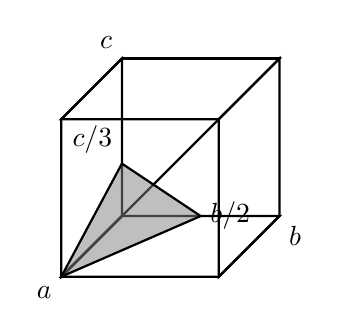
\begin{tikzpicture}[scale=1]

% Define coordinates for the cuboid
\coordinate (a) at (0,0,0); 
\coordinate (b) at (2,0,0);
\coordinate (c) at (0,2,0);
\coordinate (d) at (0,0,2);
\coordinate (e) at (2,0,2);
\coordinate (f) at (0,2,2);
\coordinate (g) at (2,2,0);
\coordinate (h) at (2,2,2);

% Draw cuboid edges
\draw[thick,black] (a) -- (b) -- (e) -- (d) -- cycle; % Bottom face
\draw[thick,black] (a) -- (c) -- (f) -- (d) -- cycle; % Left face
\draw[thick,black] (b) -- (g) -- (h) -- (e) -- cycle; % Right face
\draw[thick,black] (c) -- (g) -- (h) -- (f) -- cycle; % Top face
\draw[thick,black] (a) -- (b);
\draw[thick,black] (c) -- (g);
\draw[thick,black] (d) -- (h);

% Define triangle vertices
\coordinate (p1) at (0,0,2);    % Point 1 (0,0,2)
\coordinate (p2) at (0,2/3,0);  % Point 2 (0,2/3,0)
\coordinate (p3) at (1,0,0);    % Point 3 (1,0,0)

% Draw the triangle
\fill[gray,opacity=0.5] (p1) -- (p2) -- (p3) -- cycle;

% Draw triangle edges
\draw[thick,black] (p1) -- (p2) -- (p3) -- (p1);

% Add dashed alignment lines
\draw[dashed,black] (p1) -- (d); % Align to (0,0,2)
\draw[dashed,black] (p2) -- (c); % Align to (0,2,0)
\draw[dashed,black] (p3) -- (b); % Align to (2,0,0)

% Label requested points
\node[below left] at (d) {$a$};
\node[below right] at (b) {$b$};
\node[above left] at (c) {$c$};
\node[right] at (p3) {$b/2$};
\node[above left] at (p2) {$c/3$};

\end{tikzpicture}
\end{center}



\begin{multicols}{4}
\begin{enumerate}
\item $\sbrak{632}$ 
\item $\sbrak{123}$ 
\item $\brak{632}$ 
\item $\brak{123}$ 
\end{enumerate}
\end{multicols}


\item Which one of the following curves best represents the E vs. $f\brak{E}$ behavior of the hot
end of a metal rod demonstrating Seebeck Effect? ( $f\brak{E}$ is the probability of electron
occupancy at an energy state E ; E$_F$ is the Fermi energy) 
\begin{multicols}{4}
\begin{enumerate}
\item \begin{circuitikz}[scale=0.5]
\tikzstyle{every node}=[font=\normalsize]
\draw [->, >=Stealth] (2.25,6) .. controls (2.25,8) and (2.25,8) .. (2.25,10.25) ;
\draw [->, >=Stealth] (2.25,6) .. controls (4.75,6) and (4.5,6) .. (6.75,6) ;
\draw [dashed] (2.25,8.25) .. controls (3.75,8.25) and (3.75,8.25) .. (5,8.25);
\draw [dashed] (3.5,8.25) .. controls (3.5,6.75) and (3.5,7) .. (3.5,6);
\draw [short] (2.25,7.5) .. controls (2.75,8.5) and (4,8) .. (5,9.25);
\node [font=\normalsize] at (2,9.75) {E};
\node [font=\normalsize] at (1.75,8.25) {$E_F$};
\node [font=\normalsize] at (2.25,5.75) {0};
\node [font=\normalsize] at (3.5,5.75) {0.5};
\node [font=\normalsize] at (4.75,5.75) {1};
\node [font=\normalsize] at (6.75,5.5) {f(E)};
\end{circuitikz}
\item \begin{circuitikz}[scale=0.5]
\tikzstyle{every node}=[font=\normalsize]
\draw [->, >=Stealth] (2.25,6) .. controls (2.25,8) and (2.25,8) .. (2.25,10.25) ;
\draw [->, >=Stealth] (2.25,6) .. controls (4.75,6) and (4.5,6) .. (6.75,6) ;
\draw [dashed] (2.25,8.25) .. controls (3.75,8.25) and (3.75,8.25) .. (5,8.25);
\draw [dashed] (3.5,8.25) .. controls (3.5,6.75) and (3.5,7) .. (3.5,6);
\draw [short] (2.25,9.5) .. controls (2.5,8) and (4,8.5) .. (5,7.5);
\node [font=\normalsize] at (2,9.75) {E};
\node [font=\normalsize] at (1.75,8.25) {$E_F$};
\node [font=\normalsize] at (2.25,5.75) {0};
\node [font=\normalsize] at (3.5,5.75) {0.5};
\node [font=\normalsize] at (4.75,5.75) {1};
\node [font=\normalsize] at (6.75,5.5) {f(E)};
\end{circuitikz}
\item \begin{circuitikz}[scale=0.5]
\tikzstyle{every node}=[font=\normalsize]
\draw [->, >=Stealth] (2.25,6) .. controls (2.25,8) and (2.25,8) .. (2.25,10.25) ;
\draw [->, >=Stealth] (2.25,6) .. controls (4.75,6) and (4.5,6) .. (6.75,6) ;
\draw [dashed] (2.25,8.25) .. controls (3.75,8.25) and (3.75,8.25) .. (5,8.25);
\draw [dashed] (3.5,8.25) .. controls (3.5,6.75) and (3.5,7) .. (3.5,6);
\draw [short] (2.25,8.25) .. controls (3.5,8.25) and (4.25,8.25) .. (5,8.25);
\node [font=\normalsize] at (2,9.75) {E};
\node [font=\normalsize] at (1.75,8.25) {$E_F$};
\node [font=\normalsize] at (2.25,5.75) {0};
\node [font=\normalsize] at (3.5,5.75) {0.5};
\node [font=\normalsize] at (4.75,5.75) {1};
\node [font=\normalsize] at (6.75,5.5) {f(E)};
\draw [short] (5,8.25) .. controls (5,6.75) and (5,7) .. (5,6);
\end{circuitikz}
\item \begin{circuitikz}[scale=0.5]
\tikzstyle{every node}=[font=\normalsize]
\draw [->, >=Stealth] (2.25,6) .. controls (2.25,8) and (2.25,8) .. (2.25,10.25) ;
\draw [->, >=Stealth] (2.25,6) .. controls (4.75,6) and (4.5,6) .. (6.75,6) ;
\draw [dashed] (2.25,8.25) .. controls (3.75,8.25) and (3.75,8.25) .. (5,8.25);
\draw [dashed] (3.5,8.25) .. controls (3.5,6.75) and (3.5,7) .. (3.5,6);
\draw [short] (3.5,6) -- (3.5,8.25);
\node [font=\normalsize] at (2,9.75) {E};
\node [font=\normalsize] at (1.75,8.25) {$E_F$};
\node [font=\normalsize] at (2.25,5.75) {0};
\node [font=\normalsize] at (3.5,5.75) {0.5};
\node [font=\normalsize] at (4.75,5.75) {1};
\node [font=\normalsize] at (6.75,5.5) {f(E)};
\end{circuitikz}
\end{enumerate}
\end{multicols}


\item In a typical light emitting diode (LED), which of the following type(s) of materials
is/are used? 
\begin{enumerate}
\item Indirect bandgap semiconductor with transition metal impurities 
\item Direct bandgap semiconductor 
\item Indirect bandgap semiconductor with isoelectronic impurities 
\item Indirect bandgap semiconductor without any impurity 
\end{enumerate}



\item Which of the following options is/are true for glass transition temperature T$_g$ ?

\begin{enumerate}
\item Above T$_g$ , glass transforms from an amorphous solid to a viscous liquid.
\item At T$_g$ , glass transforms from an amorphous solid to a crystalline solid. 
\item T$_g$ is dependent on the heating rate. 
\item Below T$_g$ , nucleation and growth takes place in glass.
\end{enumerate}



\item Which of the following figures schematically represent(s) either the Frenkel defect
or the Schottky defect in ionic solids? 
\begin{multicols}{4}
\begin{enumerate}
\item \begin{circuitikz}[scale=0.25]
\tikzstyle{every node}=[font=\normalsize]
\draw  (2.5,5) circle (1cm);
\draw  (5,10) circle (1cm);
\draw  (5,5) circle (1cm);
\draw  (2.5,7.5) circle (1cm);
\draw  (2.5,10) circle (1cm);
\draw  (7.5,10) circle (1cm);
\draw  (10,10) circle (1cm);
\draw  (7.5,7.5) circle (1cm);
\draw  (7.5,5) circle (1cm);
\draw  (10,7.5) circle (1cm);
\draw  (10,5) circle (1cm);
\draw  (3.75,10) circle (0.25cm);
\draw  (6.25,10) circle (0.25cm);
\draw  (8.75,10) circle (0.25cm);
\draw  (3.75,7.5) circle (0.25cm);
\draw  (6.25,7.5) circle (0.25cm);
\draw  (8.75,7.5) circle (0.25cm);
\draw  (8.75,5) circle (0.25cm);
\draw  (3.75,5) circle (0.25cm);
\end{circuitikz}
\item \begin{circuitikz}[scale=0.25]
\tikzstyle{every node}=[font=\normalsize]
\draw  (2.5,5) circle (1cm);
\draw  (5,10) circle (1cm);
\draw  (5,5) circle (1cm);
\draw  (2.5,7.5) circle (1cm);
\draw  (2.5,10) circle (1cm);
\draw  (7.5,10) circle (1cm);
\draw  (10,10) circle (1cm);
\draw  (7.5,7.5) circle (1cm);
\draw  (7.5,5) circle (1cm);
\draw  (10,7.5) circle (1cm);
\draw  (10,5) circle (1cm);
\draw  (3.75,10) circle (0.25cm);
\draw  (6.25,10) circle (0.25cm);
\draw  (8.75,10) circle (0.25cm);
\draw  (3.75,7.5) circle (0.25cm);
\draw  (6.25,7.5) circle (0.25cm);
\draw  (8.75,7.5) circle (0.25cm);
\draw  (6.25,5) circle (0.25cm);
\draw  (8.75,5) circle (0.25cm);
\draw  (3.75,5) circle (0.25cm);
\end{circuitikz}
\item \begin{circuitikz}[scale=0.25]
\tikzstyle{every node}=[font=\normalsize]
\draw  (2.5,5) circle (1cm);
\draw  (5,10) circle (1cm);
\draw  (5,7.5) circle (1cm);
\draw  (5,5) circle (1cm);
\draw  (2.5,7.5) circle (1cm);
\draw  (2.5,10) circle (1cm);
\draw  (7.5,10) circle (1cm);
\draw  (10,10) circle (1cm);
\draw  (7.5,7.5) circle (1cm);
\draw  (7.5,5) circle (1cm);
\draw  (10,7.5) circle (1cm);
\draw  (10,5) circle (1cm);
\draw  (3.75,10) circle (0.25cm);
\draw  (6.25,10) circle (0.25cm);
\draw  (8.75,10) circle (0.25cm);
\draw  (3.75,7.5) circle (0.25cm);
\draw  (6.25,7.5) circle (0.25cm);
\draw  (8.75,7.5) circle (0.25cm);
\draw  (6.25,5) circle (0.25cm);
\draw  (8.75,5) circle (0.25cm);
\end{circuitikz}
\item \begin{circuitikz}[scale=0.25]
\tikzstyle{every node}=[font=\normalsize]
\draw  (2.5,5) circle (1cm);
\draw  (5,10) circle (1cm);
\draw  (5,7.5) circle (1cm);
\draw  (5,5) circle (1cm);
\draw  (2.5,7.5) circle (1cm);
\draw  (2.5,10) circle (1cm);
\draw  (7.5,10) circle (1cm);
\draw  (10,10) circle (1cm);
\draw  (7.5,7.5) circle (1cm);
\draw  (7.5,5) circle (1cm);
\draw  (10,7.5) circle (1cm);
\draw  (10,5) circle (1cm);
\draw  (3.75,10) circle (0.25cm);
\draw  (6.25,10) circle (0.25cm);
\draw  (8.75,10) circle (0.25cm);
\draw  (3.75,7.5) circle (0.25cm);
\draw  (6.25,7.5) circle (0.25cm);
\draw  (8.75,7.5) circle (0.25cm);
\draw  (6.25,5) circle (0.25cm);
\draw  (8.5,6.25) circle (0.25cm);
\draw  (3.75,5) circle (0.25cm);
\end{circuitikz}
\end{enumerate}
\end{multicols}


\item Given that k is the first order reaction rate constant and T is the temperature in
absolute scale, the temperature dependence of rate constant is/are represented by 
\begin{multicols}{2}
\begin{enumerate}
\item \begin{circuitikz}[scale=0.5]
\tikzstyle{every node}=[font=\normalsize]
\draw [->, >=Stealth] (2.5,6) .. controls (2.5,7.5) and (2.5,7.75) .. (2.5,9.75) ;
\draw [->, >=Stealth] (2.5,6) .. controls (4.75,6) and (4.5,6) .. (6.5,6) ;
\draw [short] (3,6.25) .. controls (5.25,6.5) and (5.25,6.5) .. (5.75,8.5);
\node [font=\normalsize] at (2.25,8.5) {k};
\node [font=\normalsize] at (4.75,5.5) {T};
\end{circuitikz}
\item \begin{circuitikz}[scale=0.5]
\tikzstyle{every node}=[font=\normalsize]
\draw [->, >=Stealth] (2.5,6) .. controls (2.5,7.5) and (2.5,7.75) .. (2.5,9.75) ;
\draw [->, >=Stealth] (2.5,6) .. controls (4.75,6) and (4.5,6) .. (6.5,6) ;
\draw [short] (3.25,6.5) .. controls (3.5,8) and (3.75,8) .. (5.75,8.5);
\node [font=\normalsize] at (2.25,8.5) {k};
\node [font=\normalsize] at (4.75,5.5) {T};
\end{circuitikz}
\item \begin{circuitikz}[scale=0.5]
\tikzstyle{every node}=[font=\normalsize]
\draw [->, >=Stealth] (2.5,6) .. controls (2.5,7.5) and (2.5,7.75) .. (2.5,9.75) ;
\draw [->, >=Stealth] (2.5,6) .. controls (4.75,6) and (4.5,6) .. (6.5,6) ;
\draw [short] (3.25,6.75) .. controls (4.75,7.75) and (4.5,7.5) .. (6,8.5);
\node [font=\normalsize] at (1.75,8.5) {ln k};
\node [font=\normalsize] at (4.75,5.5) {ln T};
\end{circuitikz}
\item \begin{circuitikz}[scale=0.5]
\tikzstyle{every node}=[font=\normalsize]
\draw [->, >=Stealth] (2.5,6) .. controls (2.5,7.5) and (2.5,7.75) .. (2.5,9.75) ;
\draw [->, >=Stealth] (2.5,6) .. controls (4.75,6) and (4.5,6) .. (6.5,6) ;
\draw [short] (3,8.5) .. controls (4.5,7.5) and (4.25,7.5) .. (5.5,6.75);
\node [font=\normalsize] at (1.75,8.5) {ln k};
\node [font=\normalsize] at (4.75,5.5) {ln T};
\end{circuitikz}
\end{enumerate}
\end{multicols}


\item For chemical vapour deposition (CVD) process, which of the following statements
is/are correct? 

\begin{enumerate}
\item Target material is stripped off by the bombardment of positive ions 
\item Source material is vapourized and thermally decomposed 
\item Partial hydrolysis of alkoxide in water solvent 
\item Suitable for preparing films of high density and uniform thickness 
\end{enumerate}



\item At room temperature, the electrical conductivity and electron mobility for aluminum are $3.8 x 10^7 (\Omega \text{m})-1 \text{ and } 0.0012 \text{m}^2 {V s}^{-1}$ , respectively. Density of free electrons for aluminum at room temperature is (in units of m$^{-3}$)  \rule{1cm}{0.4 pt} $x 10^{27}$(rounded off to nearest integer). Given: Electrical charge on an electron is $1.6 x 10^{-19}$ C. 


\item A $2$mm thick palladium sheet of $1000$mm$^2$ cross-section is used as a diffusional membrane to purify hydrogen. The hydrogen concentration is maintained at a steady state with $c_h = 1.5 \text{kg} {\text{m}}^{-3}$ and $c_l = 0.3\text{kg} {\text{m}}^{-3}$ on the two sides of the membrane as shown in the figure below.
\begin{center}
\begin{circuitikz}
\tikzstyle{every node}=[font=\normalsize]
\draw [short] (3.75,8.5) .. controls (3.75,6.25) and (3.75,6.5) .. (3.75,4.75);
\draw [short] (6.25,8.5) .. controls (6.25,6.25) and (6.25,6.5) .. (6.25,4.75);
\draw [short] (3.75,7.75) .. controls (5.25,6.75) and (5,6.75) .. (6.25,6);
\draw [short] (3.75,7.75) .. controls (3.25,7.75) and (3.5,7.75) .. (3.25,7.75);
\draw [short] (6.25,6) .. controls (6.5,6) and (6.5,6) .. (6.75,6);
\draw [<->, >=Stealth] (3.75,4.5) .. controls (5.25,4.5) and (5,4.5) .. (6.25,4.5);
\node [font=\normalsize] at (2.75,7.75) {$C_h$};
\node [font=\normalsize] at (2.75,6.5) {$Impure H_2$};
\node [font=\normalsize] at (5,4) {2 mm};
\node [font=\normalsize] at (7,6.5) {$Purer H_2$};
\node [font=\normalsize] at (7,6) {$C_l$};
\node [font=\normalsize] at (5,5.75) {Palladium};
\node [font=\normalsize] at (5,5.25) {membrane};
\end{circuitikz}
\end{center}

The rate of hydrogen purification is (in units of kg  hr$^{-1}$ \rule{1cm}{0.4 pt} $\times 10^{-6}$ (rounded off to one decimal place).\\
The diffusion coefficient of hydrogen in palladium is $1.0 \times 10^{-8} \text{m}^2 \text{s}^{-1}$.

\item In X-ray powder diffraction pattern obtained from a face centered cubic (FCC) metal, the first five reflections are at $\theta = 21.65\degree, 25.21\degree, 37.06\degree , x\text{ and } 47.58\degree.$ The
Bragg angle, $\theta$ of the fourth reflection is missed out and is represented by $x$. The
value of $x$ is (in degree) \rule{1cm}{0.4 pt} (rounded off to one decimal place). 

\item Consider a unidirectionally aligned continuous glass fibre reinforced epoxy
composite with $40$ vol. \%  reinforcement. The elastic modulus of the composite along the fibre direction is (in units of GPa) \rule{1cm}{0.4 pt} (rounded off to one decimal place).\\
Given: Elastic modulus of epoxy is $6.9$ GPa and that of glass fibre is $69$ GPa. 




